\documentclass[a4paper,12pt]{article} % добавить leqno в [] для нумерации слева
\usepackage[a4paper,top=1.3cm,bottom=2cm,left=1.5cm,right=1.5cm,marginparwidth=0.75cm]{geometry}
%%% Работа с русским языком
\usepackage{cmap}					% поиск в PDF
\usepackage[warn]{mathtext} 		% русские буквы в фомулах
\usepackage[T2A]{fontenc}			% кодировка
\usepackage[utf8]{inputenc}			% кодировка исходного текста
\usepackage[english,russian]{babel}	% локализация и переносы
\usepackage{physics}
\usepackage{multirow}

%%% Нормальное размещение таблиц (писать [H] в окружении таблицы)
\usepackage{float}
\restylefloat{table}

\usepackage{graphicx}

\usepackage{wrapfig}
\usepackage{tabularx}

\usepackage{hyperref}
\usepackage[rgb]{xcolor}
\hypersetup{
	colorlinks=true,urlcolor=blue
}

%%% Дополнительная работа с математикой
\usepackage{amsmath,amsfonts,amssymb,amsthm,mathtools} % AMS
\usepackage{icomma} % "Умная" запятая: $0,2$ --- число, $0, 2$ --- перечисление

%% Номера формул
%\mathtoolsset{showonlyrefs=true} % Показывать номера только у тех формул, на которые есть \eqref{} в тексте.

%% Шрифты
\usepackage{euscript}	 % Шрифт Евклид
\usepackage{mathrsfs} % Красивый матшрифт
\usepackage{pgfplots}
\pgfplotsset{compat=1.9}

%% Свои команды
\DeclareMathOperator{\sgn}{\mathop{sgn}}

%% Перенос знаков в формулах (по Львовскому)
\newcommand*{\hm}[1]{#1\nobreak\discretionary{}
	{\hbox{$\mathsurround=0pt #1$}}{}}

\date{\today}

\begin{document}

\begin{titlepage}
	\begin{center}
		{\large МОСКОВСКИЙ ФИЗИКО-ТЕХНИЧЕСКИЙ ИНСТИТУТ (НАЦИОНАЛЬНЫЙ ИССЛЕДОВАТЕЛЬСКИЙ УНИВЕРСИТЕТ)}
	\end{center}
	\begin{center}
		{\large Физтех-школа прикладной математики и информатики}
	\end{center}
	
	
	\vspace{4.5cm}
	{\huge
		\begin{center}
			{\bf Отчёт о выполнении лабораторной работы 4.2.1}\\
			Кольца Ньютона
		\end{center}
	}
	\vspace{1cm}
	\begin{center}
		{\large Соболевский Федор Александрович \\
                    Суходолов Олег Андреевич \\
			\vspace{0.2cm}
			Б05-111}
	\end{center}
	\vspace{8cm}
	\begin{center}
		Март 2023
	\end{center}
\end{titlepage}

\section{Аннотация}

В данной работе рассмотрено явление интерференции в тонких плёнках на примере колец Ньютона. Результаты количественных измерений в данном опыте применены для вычисления радиуса кривизны тонкой линзы интерференционным методом. На основе полученных значений и их погрешностей оценена точность данного метода.

\section{Теоретические сведения}

Явление \textit{интерференции} возникает при падении двух или более когерентных электромагнитных волн~-- волн, разность фаз которых постоянна во времени и которые при сложении дают колебания постоянной частоты. Легче всего интерференция наблюдается при сложении двух монохроматических световых волн, исходящих изначально от одного источника. Интенсивность результирующей волны $I$ при этом определяется выражением
\begin{equation} \label{interference}
    I = 2I_0 \left( 1 + \cos \frac{2\pi}{\lambda}\Delta \right),
\end{equation}
где $I_0$~-- амплитуда интерферирующих волн, $\lambda$~-- длина волны, $\Delta = n_1r_1 - n_2r_2$~-- оптическая разность хода. Из \eqref{interference} видно, что максимум интенсивности достигается, когда в разность хода укладывается целое число длин волн, т.\,е.
\begin{equation}\label{maxInt}
    \Delta = m\lambda,\quad m \in \mathbb{N}.
\end{equation}
Для условия минимумов аналогично получаем
\begin{equation}\label{minInt}
    \Delta = (m + \frac{1}{2})\lambda,\quad m \in \mathbb{N}.
\end{equation}

\textbf{Кольца Ньютона}~-- классический опыт по наблюдению интерференции, возникающей при сложении волн, отражённых от границ тонкой воздушной прослойки между сферической поверхностями линзы и тонкой стеклянной пластинки (см. рис. \ref{NewtonRings}). При нормальном падении света интерференционная картина локализована на сферической поверхности линзы и состоит из полос равной толщины.
\begin{figure}[h]
    \centering
    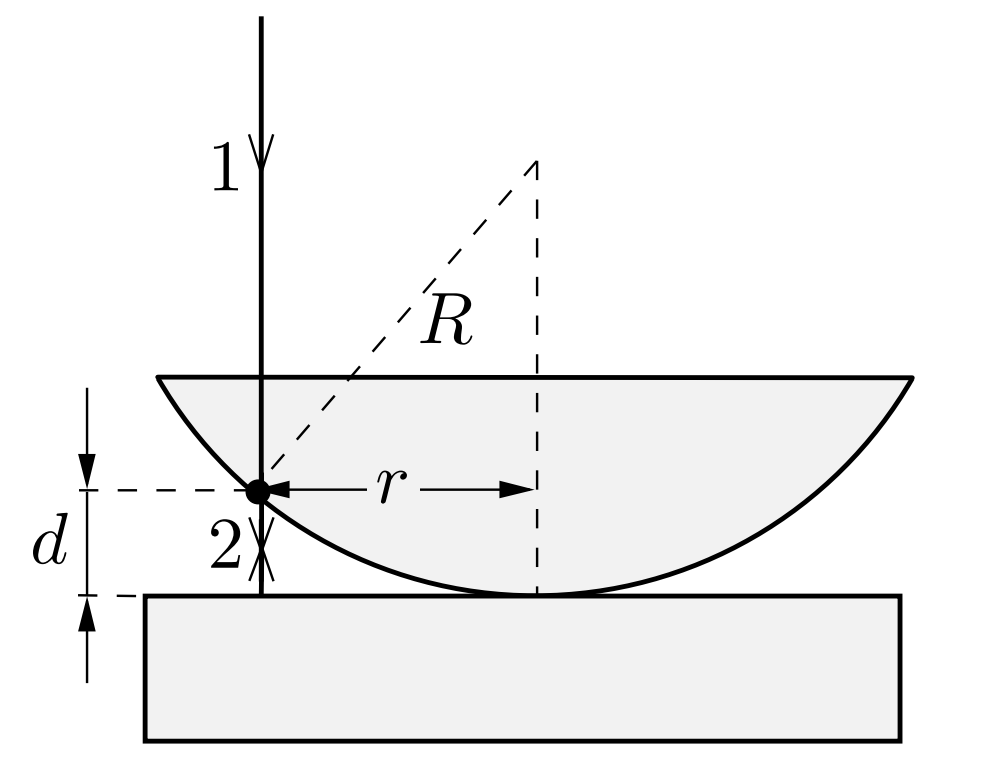
\includegraphics[width=0.5\textwidth]{NewtonRings.png}
    \caption{Схема наблюдения колец Ньютона}
    \label{NewtonRings}
\end{figure}
Оптической разностью хода в данном случае является удвоенная толщина воздушной прослойки $2d$. Для точки сферической поверхности на расстоянии $r$ от оси системы $R^2 = r^2 + (R - d)^2$. Если линза тонкая, т.\,е. $R\gg r$, то $d = r^2/2R$. При преломлении световой волны на границе воздух-стелко фаза колебаний изменяется на $\pi$, откуда оптическая разность хода
\begin{equation}\label{strokeDiff}
    \Delta = 2d + \frac{\lambda}{2} = \frac{r^2}{R} + \frac{\lambda}{2}.
\end{equation}

Из условия интерференционного минимума \eqref{minInt} и \eqref{strokeDiff} получаем радиусы тёмных колец:
\begin{equation}\label{DarthRadius}
    r_m = \sqrt{2mR\lambda}.
\end{equation}
Аналогично, из \eqref{maxInt} получаются радиусы светлых колец:
\begin{equation}
    r'_m = \sqrt{(2m-1)R\lambda}.
\end{equation}

\section{Методика измерений}

\textbf{В работе использовались:} измерительный микроскоп с опак-иллюминатором; плосковыпуклая линза; пластинка из чёрного стекла; ртутная лампа; линзы; цветные фильтры; объектная шкала.
\begin{figure}[h]
    \centering
    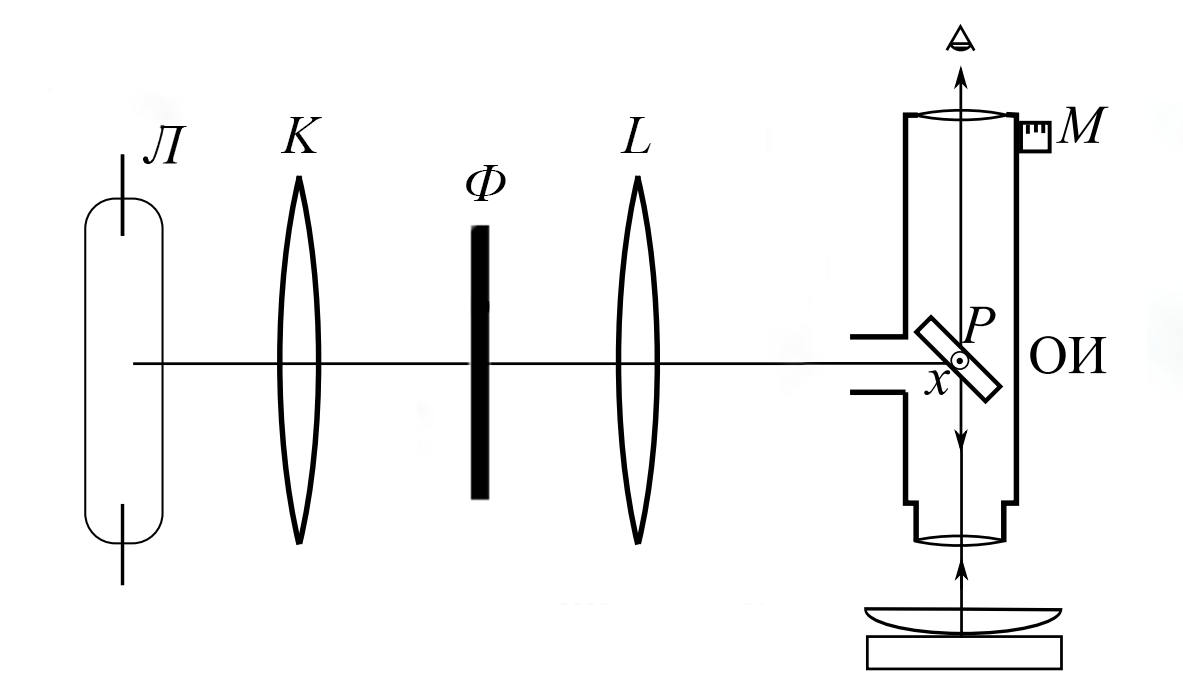
\includegraphics[width=0.7\textwidth]{setup.png}
    \caption{Схема экспериментальной установки}
    \label{setup}
\end{figure}

Схема экспериментальной установки изображена на рис. \ref{setup}. Свет из лампы \textit{Л}, проходя через цветной фильтр, фокусируется с помощью двух линз \textit{K} и \textit{L} в отверстие опак-иллюминатора ОИ микроскопа. С помощью отражающей пластинки \textit{P} свет направляется на линзу, закреплённую на пластинке. Размеры колец измеряются при помощи окулярной шкалы и микрометрического винта \textit{M}. Для градуировки измерительной шкалы объектива используется проградуированная микрометрическая объектная шкала.

В работе были исследованы кольца Ньютона, возникающие при монохроматическом и дихроматическом освещении. В первом случае использовался оранжевый фильтр с длиной волны $\lambda = 579$ нм, во втором~-- жёлто-зелёный, пропускающий свет с длинами волн $\lambda_1 = 546$ нм и $\lambda_2 = 579$ нм. Во втором эксперименте при наложении друг на друга двух интерференционных картин наблюдались так называемые <<биения>>~-- светлые и тёмные полосы то чередуются, то совпадают. По расстоянию между совпадающими тёмными полосами можно экспериментально определить отношение длин волн $\lambda_1$ и $\lambda_2$ и таким образом оценить точность формулы \eqref{DarthRadius}. 

\section{Результаты экспериментов}

После юстировки экспериментальной установки были получены картины колец Ньютона
для каждого из фильтров. Картина для жёлто-зелёного фильтра изображена на рис. \ref{ringImage}. Для длины волны $\lambda = 579$ нм были измерены радиусы первых десяти тёмных колец в делениях измерительной шкалы. Затем было установлено, что одно деление измерительной шкалы совпадает с большим делением объектной шкалы и имеет длину 0,1 мм. 
\begin{figure}[h]
    \centering
    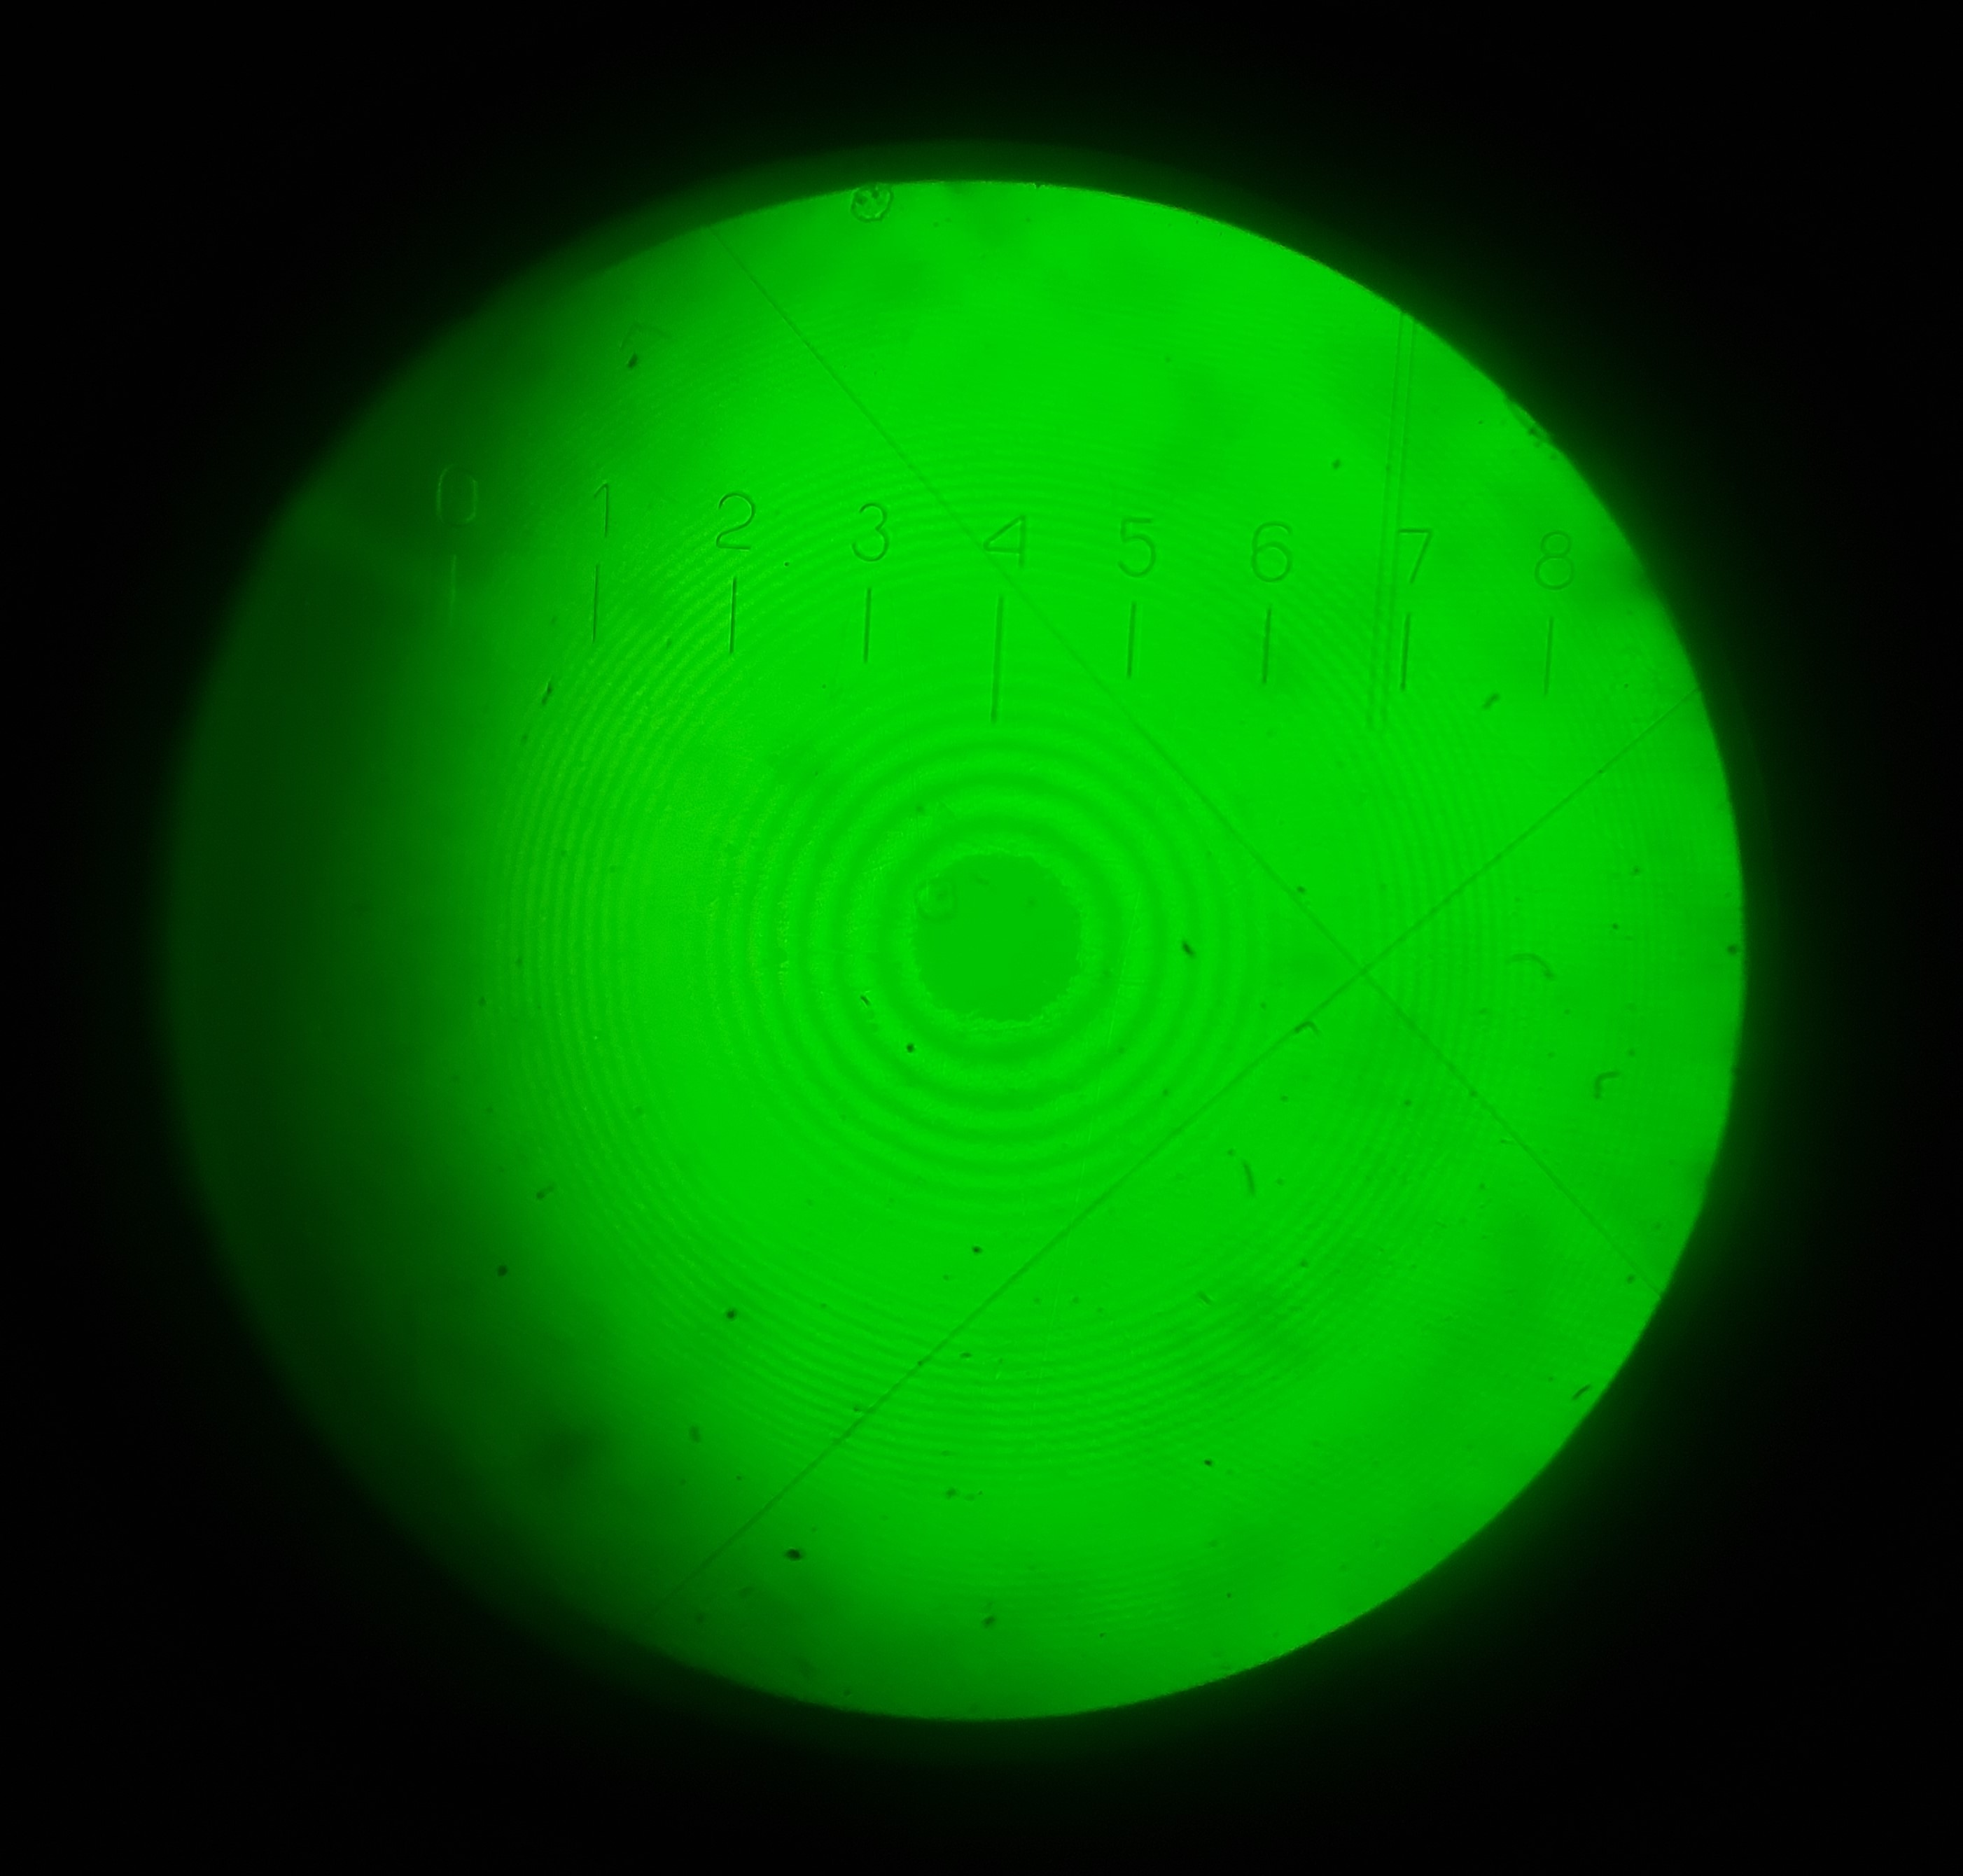
\includegraphics[width=0.4\textwidth]{rings.jpg}
    \caption{Кольца Ньютона для двух длин волн}
    \label{ringImage}
\end{figure}

Результаты измерения радиусов колец приведены в таблице \ref{radii}. На графике \ref{graph} представлена зависимость квадрата радиуса кольца $r_m^2$ от его номера $m$. Методом наименьших квадратов определены:
\begin{itemize}
    \item коэффициент наклона $k = 2R\lambda = 1,488\cdot 10^{-2}$ мм$^2$;
    \item случайная погрешность $\sigma_k^\text{случ} = 0,004\cdot 10^{-2}$ мм$^2$.
\end{itemize}
\begin{table}[h]
    \centering
    \begin{tabular}{|c|c|c|} \hline
        $m$ & $r_m$, дел & $r_m^2$, $10^{-2}$ мм$^2$ \\ \hline
        1 & 0,91 & 0,83 \\ \hline
        2 & 1,24 & 1,54 \\ \hline
        3 & 1,51 & 2,28 \\ \hline
        4 & 1,74 & 3,03 \\ \hline
        5 & 1,93 & 3,72 \\ \hline
        6 & 2,11 & 4,45 \\ \hline
        7 & 2,29 & 5,24 \\ \hline
        8 & 2,44 & 5,95 \\ \hline
        9 & 2,58 & 6,66 \\ \hline
        10& 2,72 & 7,40 \\ \hline
    \end{tabular}
    \caption{Радиусы колец}
    \label{radii}
\end{table}

\begin{figure}[h] \label{graph}
\begin{center}
\begin{tikzpicture}
    \begin{axis}[
    xlabel={Номер кольца $m$},
    ylabel={$r_m^2$, $10^{-2}$ мм$^2$},
    xmajorgrids=true,
    ymajorgrids=true,
    grid style=dashed,
    xmin = 0,
    ymin = 0,
    xmax = 10.5,
    ymax = 8.5
    ]
    \addplot[color=black, mark=x, only marks] coordinates{
    (1, 0.83)
    (2, 1.54)
    (3, 2.28)
    (4, 3.03)
    (5, 3.72)
    (6, 4.45)
    (7, 5.24)
    (8, 5.95)
    (9, 6.66)
    (10, 7.40)
    };
    \addplot[color=blue, domain=0:11]{x*0.743};
    \end{axis}
\end{tikzpicture}
\caption{Зависимость радиуса тёмного интерференционного кольца от его номера}
\end{center}
\end{figure}

С учётом систематической погрешности $\Delta_k^\text{сист} = 0,002\cdot 10^{-2}$ мм$^2$, полная погрешность $\sigma_k = 0,005\cdot 10^{-2}$ мм$^2$.
Зная $k$ и $\lambda$, можно определить радиус кривизны линзы $R$:
$$
R = \frac{k}{\lambda} = 2,570 \pm 0,013 \text{ см}.
$$
Получено значение с относительной погрешностью 0,5\%.

В ходе опыта с двухполосным фильтром (см. рис. \ref{ringImage}) было установлено, что тёмные полосы двух интерференционных картин точно совпадают через $\Delta m = 18$ полос. Из формулы \eqref{radii} получаем соотношение:
$$
\frac{\Delta m - 1}{\Delta m} = \frac{\lambda_1}{\lambda_2} = \frac{17}{18} \approx 0.944.
$$
С использованием указанных значений $\lambda_1$ и $\lambda_2$ получается значение $\lambda_1/\lambda_2 = 0,943$, что практически совпадает со значением, вычисленным по формуле (погрешность менее 0,1\%).

\section{Выводы}
В ходе работы удалось пронаблюдать возникновение колец Ньютона в результате интерференции в тонких плёнках. Приближения, которыми мы пользовались при выводе формул для колец Ньютона (например, пренебрежение преломлением лучей на границе стекло-воздух), можно считать оправданными, так как отношение длин волн, полученное численно из наблюдаемых при дихроматическом освещении биений, с точностью до десятой доли процента совпадает со значением, полученным из справочных данных. Погрешность определения радиуса линзы, для сравнения, оказалась в пять раз больше~-- около половины процента.

Столь малое значение погрешности определения радиуса линзы позволяют утверждать, что для линз малых размеров интерференционный метод определения радиуса кривизны является предпочтительным относительно, например, методов геометрической оптики. Для сравнения можно взять результат из лабораторной работы 4.1.1: фокусные расстояния использованных в ней линз удалось определить с точностью не более 15\% процентов, что на несколько порядков ниже, чем в данной работе. Такие погрешности возникали вследствие аббераций и неидеальной юстировки оптической системы. В данной же работе эти проблемы не были существенны.

\end{document}